\chapter{Implementation}

\section{Overview}
This chapter shows how the project was implemented in a more-detailed way. It also shows some of the key points for this application, how they were implemented and what they are useful for. This chapter of the documentation is the technical part of it.\\
It will show how the data is inserted into the server, how it is processed and based on the request, how that data is used to return a response to that specific request.\\
This section will also cover some of the important techniques that were used for example to test, to document, to generate artifacts etc. It will also cover the code repository and CI/CD part, which for this application, is  \href{https://gitlab.com/}{GitLab}.

\section{API}
This application serves as an API for OAPIF clients or the driver itself. In order to use it, one must point it to the URL where it is hosted under. All the paths and request handling are taken care by the application itself. The application has around 6 API endpoints which some of them are a requirement from the "OGC API - Features" standard, and the others are a requirement for one of the front-end applications (a map of castles in Switzerland), which is going to use this API to serve features, geometry objects but also PNG raster tiles which will appear as dots in the application where a user can click on them in order to view what castle is hidden under a dot and get more information about it.\\
The application uses a library called \href{https://fastapi.tiangolo.com/}{FastAPI}, which was very convenient for this project and offers a lot of different ways of implementing an API, depending on the requirements and the nature of the application.\\
\newline
FastAPI is a modern, fast (high-performance), web framework for building APIs with Python 3.6+ based on standard Python type hints.

The key features are:
\begin{itemize}
\item Fast: Very high performance, on par with NodeJS and Go (thanks to Starlette and Pydantic). One of the fastest Python frameworks available.

\item Fast to code: Increase the speed to develop features by about 200% to 300% *.

\item Fewer bugs: Reduce about 40% of human (developer) induced errors. *
\item Intuitive: Great editor support. Completion everywhere. Less time debugging.
\item Easy: Designed to be easy to use and learn. Less time reading docs.
\item Short: Minimize code duplication. Multiple features from each parameter declaration. Fewer bugs.
\item Robust: Get production-ready code. With automatic interactive documentation.
\item Standards-based: Based on (and fully compatible with) the open standards for APIs: OpenAPI (previously known as Swagger) and JSON Schema. \cite{WhatIsFastAPI}
\end{itemize} 

\section{GeoJSON \& Features}
This application works a lot with GeoJSON. It processes it and uses various libraries to serialize/deserialize it in order to re-format it and present it to the request response in the appropriate format.\\
The application needs a GeoJSON file (.geojson) to be supplied using the environment variables in the docker compose file (multiple files can be passed too). The GeoJSON file should contain a FeatureCollection with Features inside that the server will use to display and send responses using those features. These files, when parsed and formatted appropriately are called \textit{collections} in the application and in the \textit{OGC API - Features} standard.\\
\newline
GeoJSON is a geospatial data interchange format based on JavaScript
Object Notation (JSON).  It defines several types of JSON objects and
the manner in which they are combined to represent data about
geographic features, their properties, and their spatial extents.
GeoJSON uses a geographic coordinate reference system, World Geodetic
System 1984, and units of decimal degrees. \cite{WhatIsGeoJSON}\\
\newpage
A Feature object represents a spatially bounded thing.  Every Feature
object is a GeoJSON object no matter where it occurs in a GeoJSON
text.
\begin{itemize}
\item A Feature object has a "type" member with the value "Feature".
\item A Feature object has a member with the name "geometry". The value
of the geometry member SHALL be either a Geometry object as
defined above or, in the case that the Feature is unlocated, a
JSON null value.
\item A Feature object has a member with the name "properties".  The
value of the properties member is an object (any JSON object or a
JSON null value). \cite{WhatIsGeoJSON}\\
\newline

Here's an example of some minimal GeoJSON data:

\begin{minted}{json}
{
  "features": [
      {
        "geometry": {
        "coordinates": [
          11.183468,
          47.910414
        ],
        "type": "Point"
      },
        "id": "N123",
        "properties": {
        "natural": "lake",
        "name": "Katzensee"
      },
      "type": "Feature"
      }
  ],
  "type": "FeatureCollection"
}
\end{minted}
\end{itemize}

\section{Raster Tiles}


\section{Testing}
This application has two testing methods integrated. That is the Unit Testing which was done using \href{https://docs.pytest.org/en/latest/}{pytest} and the Load Testing part which was done using \href{https://locust.io/}{Locust}.\\
The Unit Testing was done to test some of the main features of the application, some HTTP requests \& responses etc.\\
The Load Testing was done to test what happens if a lot of users access the server and make the same requests at the same time, what the performance of the server into giving responses would be.
\subsection{Unit Testing}
The Unit Testing, as said above, was done by using \href{https://docs.pytest.org/en/latest/}{pytest}.\\
Unit Testing is a software testing method where individual parts of the code, or modules, or usage procedures are tested in order to find out if they work as expected.\\
pytest is a framework that makes building simple and scalable tests easy. Tests are expressive and readable—no boilerplate code required. \cite{WhatIsPytest}	
pytest is a more "pythonic" way of unit testing in Python. It uses the native Python syntax and methods in order to assert results. After all the unit tests are created, they can be simply run with the command:
\begin{minted}{bash}
$ pytest <path of file or path of folder>
\end{minted}
What this will do is will check all the files within that directory or the file itself if it is a file and test them all, if one of them fails it will show which one and return a failure error, if all of them succeed it will say all of them succeeded and will pass the unit tests.\\
\newline
An example of a unit test using pytest:
\begin{minted}{python}
# content of test_class.py
class TestClass:
  def inc(x):
    return x + 1

  def test_answer():
    assert inc(3) == 5
\end{minted}
\newpage
This will return a failure, because 3 + 1  is equal to 4 and not to 5:
\begin{minted}{bash}
$ pytest
=========================== test session starts ============================
platform linux -- Python 3.x.y, pytest-5.x.y, py-1.x.y, pluggy-0.x.y
cachedir: $PYTHON_PREFIX/.pytest_cache
rootdir: $REGENDOC_TMPDIR
collected 1 item

test_sample.py F                                                     [100%]

================================= FAILURES =================================
_______________________________ test_answer ________________________________

def test_answer():
>       assert inc(3) == 5
E       assert 4 == 5
E        +  where 4 = inc(3)

test_sample.py:6: AssertionError
============================ 1 failed in 0.12s =============================
\end{minted}

And in this project's case, for example, where all the unit tests succeed, it shows this:
\begin{minted}{bash}
$ pytest tests/
============================ test session starts ============================ 
platform win32 -- Python 3.7.4, pytest-5.2.2, py-1.8.0, pluggy-0.13.0
rootdir: C:path\to\directory\python-wfs-server
collected 22 items                                                                                                                                                                                               

tests\test_geometry.py ....                                                                                                                                                                                [ 18%]
tests\test_index.py ...                                                                                                                                                                                    [ 31%]
tests\test_server.py .............                                                                                                                                                                         [ 90%]
tests\test_tiles.py ..                                                                                                                                                                                     [100%]

============================ 22 passed in 1.36s ============================ 
\end{minted}
\newpage
\subsection{Load Testing}
The Load Testing part, was done using \href{https://locust.io/}{Locust}.\\
Load testing is a subset of performance testing, it puts demand on a system and measures its response time and performance. It is used to check how a system behaves under low, normal or peak load conditions.\\
Locust is an easy-to-use, distributed, user load testing tool. It is intended for load-testing web sites (or other systems) and figuring out how many concurrent users a system can handle.\\
The idea is that during a test, a swarm of locusts will attack your website. The behavior of each locust (or test user if you will) is defined by you and the swarming process is monitored from a web UI in real-time. This will help you battle test and identify bottlenecks in your code before letting real users in. \cite{WhatIsLocust}\\
\newline
A locust file looks something like this:
\begin{minted}{python}
from locust import HttpLocust, TaskSet, between

def login(l):
  l.client.post("/login", {"username":"ellen_key", "password":"education"})

def logout(l):
  l.client.post("/logout", {"username":"ellen_key", "password":"education"})

def index(l):
  l.client.get("/")

def profile(l):
  l.client.get("/profile")

class UserBehavior(TaskSet):
  tasks = {index: 2, profile: 1}

def on_start(self):
  login(self)

def on_stop(self):
  logout(self)

class WebsiteUser(HttpLocust):
  task_set = UserBehavior
  wait_time = between(5.0, 9.0)
\end{minted}
To run locust, we just simply run the command:
\begin{minted}{bash}
$ locust
\end{minted}
After that, the locust server starts and can be accessed by default in \href{ http://127.0.0.1:8089}{http://127.0.0.1:8089} (if Locust is being ran locally). Then a page would open that would look something like this:
\begin{figure}[H]
	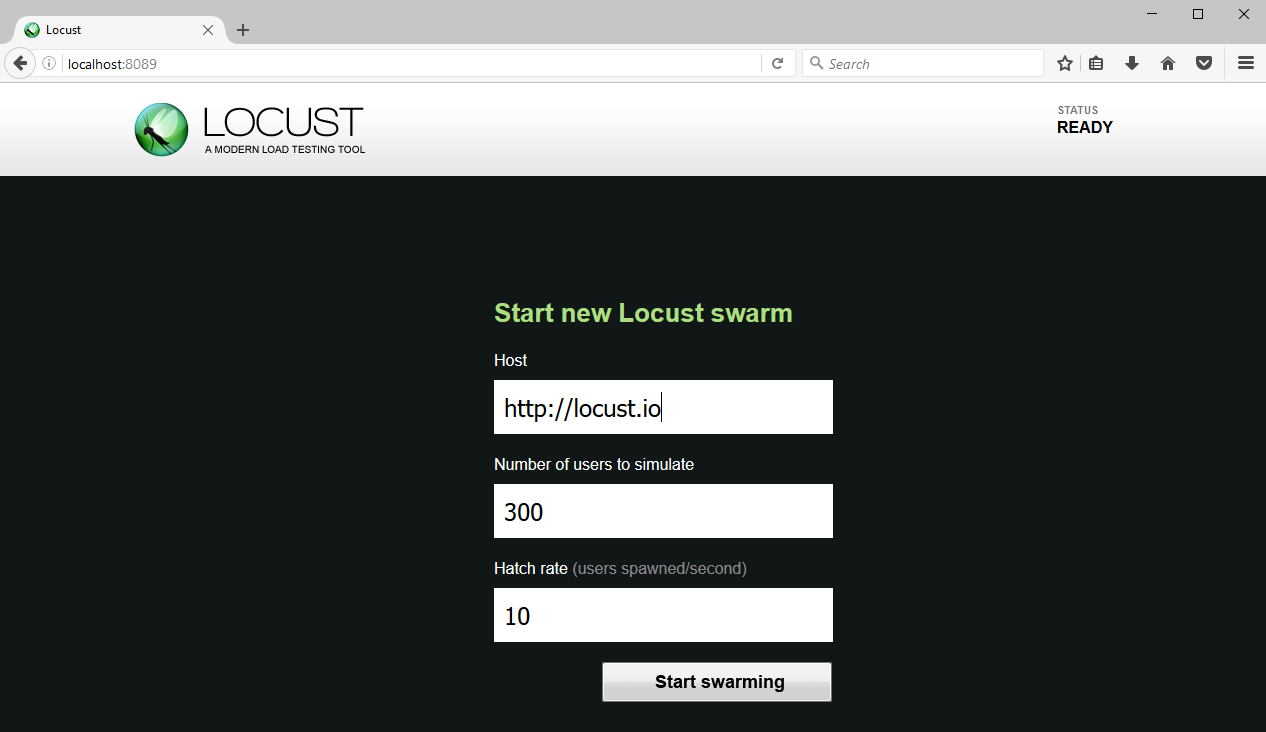
\includegraphics[width=\linewidth]{./Images/Implementation/locust_interface.png}
	\caption{A look at the Locus web-interface}
\end{figure}
\newpage
\section{GitLab}
The code repository and CI/CD for this project were provided by \href{https://gitlab.com/}{GitLab}.\\
GitLab is a DevOps lifecycle tool that provides a lot of things like: Git-repository manager providing wiki, issue-tracking and CI/CD pipeline features, it uses an open-source license and is developed by \href{https://about.gitlab.com/company/}{GitLab Inc}.
It has a very nice web interface and lots of different features that make application lifecycle much easier. The features GitLab offers that were used for this project were the project repository and the CI/CD feature.\\
\newline
CI/CD, or continuous integration and continuous delivery (aka continuous deployment), combines the values of these two practices in order to provide precise integration and delivery.
GitLab has a feature of writing a CI/CD file which does various operations for you each and every push, to make sure that the CI/CD logic still works with the applied changes.\\
In this case, CI/CD was used to test the project (run the unit tests), to compile the LaTeX document, retrieve a PDF out of it and then generate and upload that PDF into an artifact which can be downloaded from the CI/CD pipeline.
\begin{figure}[H]
	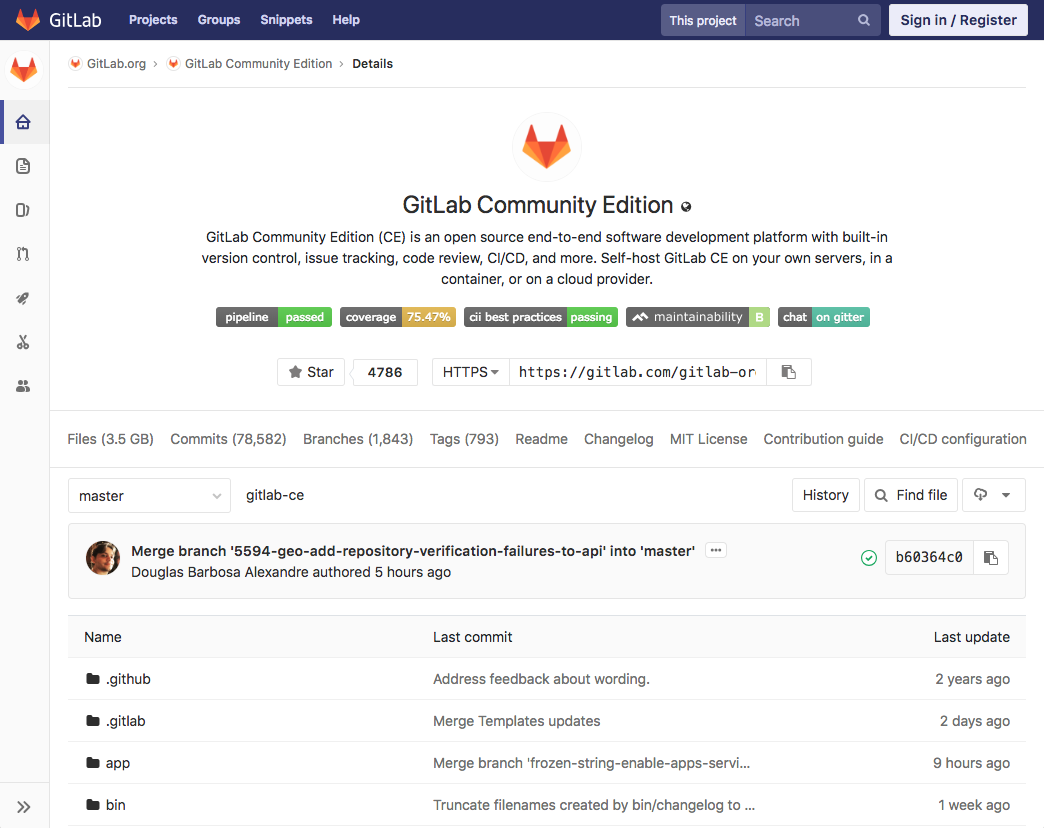
\includegraphics[width=\linewidth]{./Images/Implementation/gitlab_view.png}
	\caption{A peek at the GitLab interface}
\end{figure}	
\section{LaTeX}
The system that was used in order to document this project was \href{https://www.LaTeX-project.org/}{LaTeX}.\\
LaTeX is a high-quality typesetting system; it includes features designed for the production of technical and scientific documentation. LaTeX is the de facto standard for the communication and publication of scientific documents. LaTeX is available as free software. \cite{WhatIsLaTeX}\\
The application that was used in conjunction with LaTeX was \href{http://texstudio.sourceforge.net/}{TeXstudio}.
TeXstudio is an integrated writing environment for creating LaTeX documents. Our goal is to make writing LaTeX as easy and comfortable as possible. Therefore TeXstudio has numerous features like syntax-highlighting, integrated viewer, reference checking and various assistants. \cite{WhatIsTeXStudio}\\
The reason why LaTeX was used is that it is very convenient to developers, since they can get used to the syntax very quickly and are familiar with "coding" approaches. Another big reason is that it provides a lot of packages for displaying code in a nice formatted way, it has the ability of displaying web links in a nice manner and also the figures and figure alignments are very appropriate and easy to create \& maintain.\\
\newline
This is how a portion of this page for example looks like in LaTeX before being compiled:
\begin{minted}[linenos,tabsize=2,breaklines]{latex}
\section{LaTeX}
The system that was used in order to document this project was \href{https://www.LaTeX-project.org/}{LaTeX}.\\
LaTeX is a high-quality typesetting system; it includes features designed for the production of technical and scientific documentation. LaTeX is the de facto standard for the communication and publication of scientific documents. LaTeX is available as free software. \cite{WhatIsLaTeX}\\
The application that was used in conjunction with LaTeX was \href{http://texstudio.sourceforge.net/}{TeXstudio}.
TeXstudio is an integrated writing environment for creating LaTeX documents. Our goal is to make writing LaTeX as easy and comfortable as possible. Therefore TeXstudio has numerous features like syntax-highlighting, integrated viewer, reference checking and various assistants. \cite{WhatIsTeXStudio}\\
\end{minted}
